% Options for packages loaded elsewhere
\PassOptionsToPackage{unicode}{hyperref}
\PassOptionsToPackage{hyphens}{url}
%
\documentclass[
]{book}
\usepackage{amsmath,amssymb}
\usepackage{iftex}
\ifPDFTeX
  \usepackage[T1]{fontenc}
  \usepackage[utf8]{inputenc}
  \usepackage{textcomp} % provide euro and other symbols
\else % if luatex or xetex
  \usepackage{unicode-math} % this also loads fontspec
  \defaultfontfeatures{Scale=MatchLowercase}
  \defaultfontfeatures[\rmfamily]{Ligatures=TeX,Scale=1}
\fi
\usepackage{lmodern}
\ifPDFTeX\else
  % xetex/luatex font selection
\fi
% Use upquote if available, for straight quotes in verbatim environments
\IfFileExists{upquote.sty}{\usepackage{upquote}}{}
\IfFileExists{microtype.sty}{% use microtype if available
  \usepackage[]{microtype}
  \UseMicrotypeSet[protrusion]{basicmath} % disable protrusion for tt fonts
}{}
\makeatletter
\@ifundefined{KOMAClassName}{% if non-KOMA class
  \IfFileExists{parskip.sty}{%
    \usepackage{parskip}
  }{% else
    \setlength{\parindent}{0pt}
    \setlength{\parskip}{6pt plus 2pt minus 1pt}}
}{% if KOMA class
  \KOMAoptions{parskip=half}}
\makeatother
\usepackage{xcolor}
\usepackage{longtable,booktabs,array}
\usepackage{calc} % for calculating minipage widths
% Correct order of tables after \paragraph or \subparagraph
\usepackage{etoolbox}
\makeatletter
\patchcmd\longtable{\par}{\if@noskipsec\mbox{}\fi\par}{}{}
\makeatother
% Allow footnotes in longtable head/foot
\IfFileExists{footnotehyper.sty}{\usepackage{footnotehyper}}{\usepackage{footnote}}
\makesavenoteenv{longtable}
\usepackage{graphicx}
\makeatletter
\def\maxwidth{\ifdim\Gin@nat@width>\linewidth\linewidth\else\Gin@nat@width\fi}
\def\maxheight{\ifdim\Gin@nat@height>\textheight\textheight\else\Gin@nat@height\fi}
\makeatother
% Scale images if necessary, so that they will not overflow the page
% margins by default, and it is still possible to overwrite the defaults
% using explicit options in \includegraphics[width, height, ...]{}
\setkeys{Gin}{width=\maxwidth,height=\maxheight,keepaspectratio}
% Set default figure placement to htbp
\makeatletter
\def\fps@figure{htbp}
\makeatother
\setlength{\emergencystretch}{3em} % prevent overfull lines
\providecommand{\tightlist}{%
  \setlength{\itemsep}{0pt}\setlength{\parskip}{0pt}}
\setcounter{secnumdepth}{5}
\usepackage{booktabs}
\ifLuaTeX
  \usepackage{selnolig}  % disable illegal ligatures
\fi
\usepackage[]{natbib}
\bibliographystyle{plainnat}
\usepackage{bookmark}
\IfFileExists{xurl.sty}{\usepackage{xurl}}{} % add URL line breaks if available
\urlstyle{same}
\hypersetup{
  pdftitle={Maple},
  pdfauthor={Ashan J},
  hidelinks,
  pdfcreator={LaTeX via pandoc}}

\title{Maple}
\author{Ashan J}
\date{2024-09-15}

\usepackage{amsthm}
\newtheorem{theorem}{Theorem}[chapter]
\newtheorem{lemma}{Lemma}[chapter]
\newtheorem{corollary}{Corollary}[chapter]
\newtheorem{proposition}{Proposition}[chapter]
\newtheorem{conjecture}{Conjecture}[chapter]
\theoremstyle{definition}
\newtheorem{definition}{Definition}[chapter]
\theoremstyle{definition}
\newtheorem{example}{Example}[chapter]
\theoremstyle{definition}
\newtheorem{exercise}{Exercise}[chapter]
\theoremstyle{definition}
\newtheorem{hypothesis}{Hypothesis}[chapter]
\theoremstyle{remark}
\newtheorem*{remark}{Remark}
\newtheorem*{solution}{Solution}
\begin{document}
\maketitle

{
\setcounter{tocdepth}{1}
\tableofcontents
}
\chapter{Introduction to Maple}\label{introduction-to-maple}

Placeholder

\section{What is Maple?}\label{what-is-maple}

\section{Using a Maple Worksheet}\label{using-a-maple-worksheet}

\section{Entering Maple Commands}\label{entering-maple-commands}

\section{Arithmetic operations}\label{arithmetic-operations}

\section{Operations}\label{operations}

\subsection{Exercises}\label{exercises}

\section{Shortcut to retyping}\label{shortcut-to-retyping}

\section{Fractions and Decimals}\label{fractions-and-decimals}

\section{Roots}\label{roots}

\subsection{Exercise}\label{exercise}

\section{Pi Vs pi}\label{pi-vs-pi}

\section{Rational Numbers}\label{rational-numbers}

\subsection{Exercises}\label{exercises-1}

\section{Complex Numbers}\label{complex-numbers}

\subsection{Exercise}\label{exercise-1}

\section{MAPLE Help}\label{maple-help}

\chapter{Basic Algebra}\label{basic-algebra}

Placeholder

\section{Variables and Expressions}\label{variables-and-expressions}

\subsection{Exercise}\label{exercise-2}

\section{Assigning values to variables}\label{assigning-values-to-variables}

\section{Substituting Values}\label{substituting-values}

\section{Factoring expressions}\label{factoring-expressions}

\section{Expanding expressions}\label{expanding-expressions}

\section{Finding the degree and leading coefficient of polynomials}\label{finding-the-degree-and-leading-coefficient-of-polynomials}

\subsection{Exercise}\label{exercise-3}

\section{Simplifying Expressions}\label{simplifying-expressions}

\chapter{Matrices}\label{matrices}

Placeholder

\section{Defining matrices}\label{defining-matrices}

\subsection{Addition and Scalar Multiplication}\label{addition-and-scalar-multiplication}

\subsection{Matrix Multiplication}\label{matrix-multiplication}

\subsection{Transpose}\label{transpose}

\section{Row Opreations}\label{row-opreations}

\section{Determinanat of Matrix}\label{determinanat-of-matrix}

\subsection{Inverse of a matrix}\label{inverse-of-a-matrix}

\section{Exercise}\label{exercise-4}

\chapter{System of Linear Equations and Matrices}\label{system-of-linear-equations-and-matrices}

A linear system is a collection of first degree equations. A solution to a system consists of one or more sets of specific values that our common solutions to each of the individual equations. Here is a simple example which we can solve quite easily using the \texttt{solve} command.

\section{Augment of a matrix}\label{augment-of-a-matrix}

\begin{verbatim}
[> with(linalg):
[> A:=matrix([[1,2],[2,3]]);
\end{verbatim}

\emph{Output}:

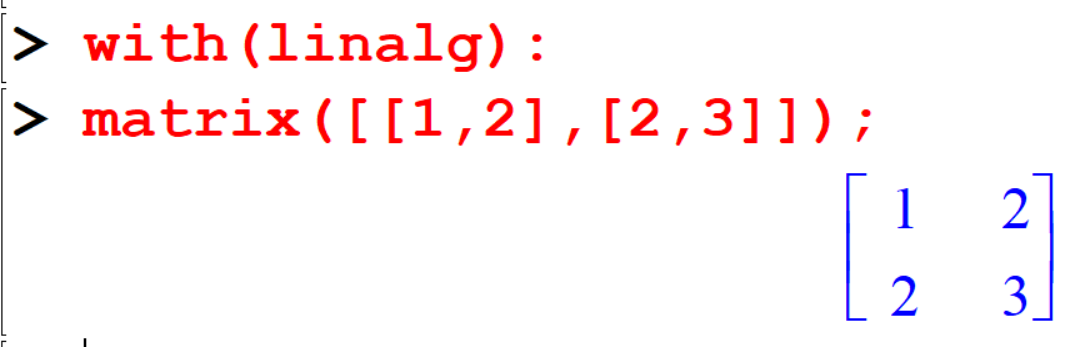
\includegraphics[width=0.6\textwidth,height=\textheight]{figures/Lesson 5/fig1.png}

\begin{verbatim}
[> B:=matrix([[3,4,5],[6,7,8]]);
\end{verbatim}

\emph{Output}:

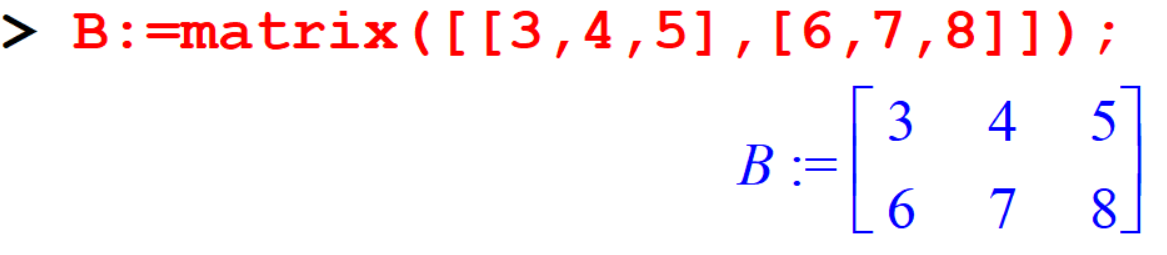
\includegraphics[width=0.6\textwidth,height=\textheight]{figures/Lesson 5/fig2.png}

\begin{verbatim}
augment(A,B);
\end{verbatim}

\emph{Output}:

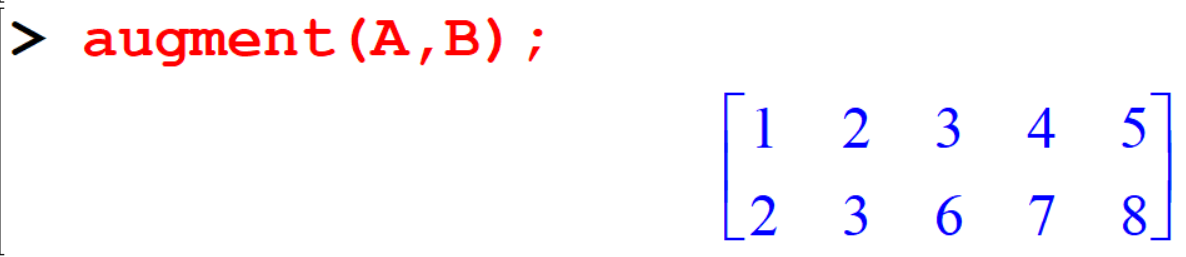
\includegraphics[width=0.6\textwidth,height=\textheight]{figures/Lesson 5/fig3.png}

The function augment joins two or more matrices together horizontally.
The matrices and vectors must have the same number of rows.

\section{Solving Linear Systems}\label{solving-linear-systems}

There are three types of systems of linear equations, and three types of solutions.

\begin{itemize}
\tightlist
\item
  An \textbf{independent system} has exactly one solution.
\item
  An \textbf{inconsistent system} has no solution.
\item
  A \textbf{dependent system} has infinitely many solutions.
\end{itemize}

\begin{longtable}[]{@{}
  >{\raggedright\arraybackslash}p{(\columnwidth - 6\tabcolsep) * \real{0.2121}}
  >{\centering\arraybackslash}p{(\columnwidth - 6\tabcolsep) * \real{0.3182}}
  >{\centering\arraybackslash}p{(\columnwidth - 6\tabcolsep) * \real{0.2121}}
  >{\centering\arraybackslash}p{(\columnwidth - 6\tabcolsep) * \real{0.2576}}@{}}
\toprule\noalign{}
\begin{minipage}[b]{\linewidth}\raggedright
---
\end{minipage} & \begin{minipage}[b]{\linewidth}\centering
Type of Linear~System
\end{minipage} & \begin{minipage}[b]{\linewidth}\centering
Independent~Systems
\end{minipage} & \begin{minipage}[b]{\linewidth}\centering
Inconsistent~Systems
\end{minipage} \\
\midrule\noalign{}
\endhead
\bottomrule\noalign{}
\endlastfoot
No of Solution & Exactly one solution & No solution & Infinitely many solutions \\
Example 1 & \(\begin{aligned}x - 3y &=-3\\2x + y &= 8\end{aligned}\) & \(\begin{aligned}x - 3y &= - 3\\x -y &=3\end{aligned}\) & \(\begin{aligned}x - 3y &= - 3\\2x + 6y &= -6 \end{aligned}\) \\
& 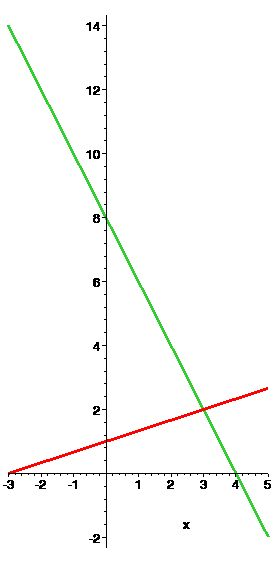
\includegraphics{figures/Lesson 5/1.jpg} & 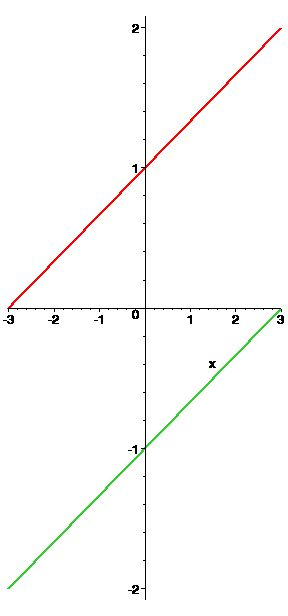
\includegraphics{figures/Lesson 5/2.jpg} & 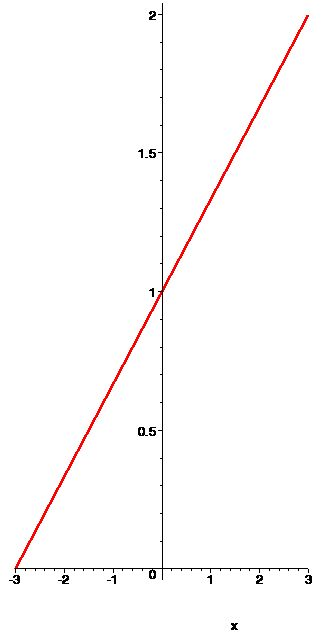
\includegraphics{figures/Lesson 5/3.jpg} \\
Example 2 & \(\begin{aligned}x+y+z&=2\\
6x-4y+5z&=1\\
5x+2y+2z&=3\end{aligned}\) & \(\begin{aligned}x-3y+z&=4\\-y-4z&=7\\2y+8z&=24 \end{aligned}\) & \(\begin{aligned}2x+y-3z&=0\\
4x+2y-6z&=0\\
x-y+z&=0\end{aligned}\) \\
& 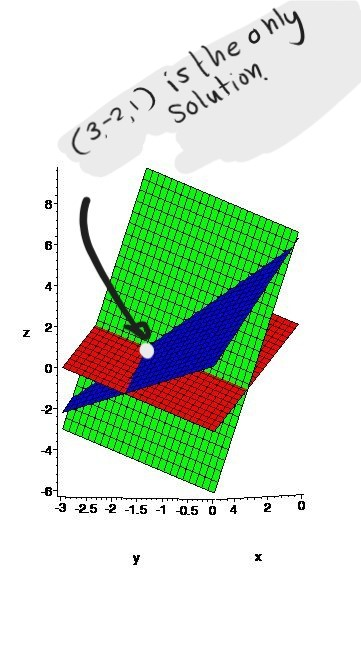
\includegraphics{figures/Lesson 5/23.jpg} & 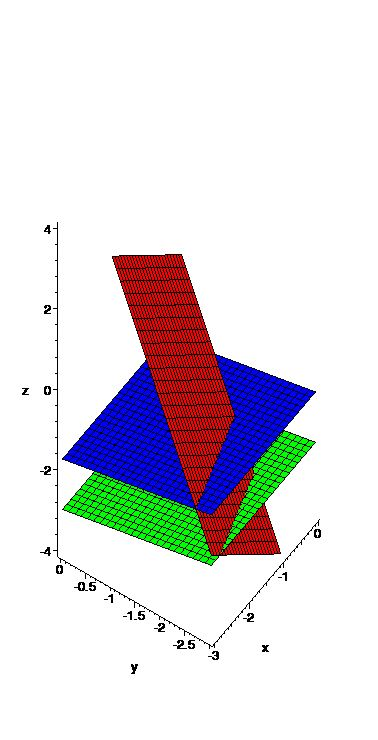
\includegraphics{figures/Lesson 5/22.jpg} & 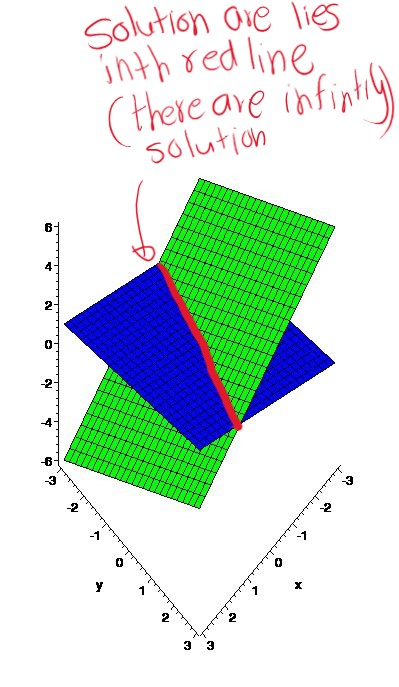
\includegraphics{figures/Lesson 5/21.jpg} \\
\end{longtable}

Let's try to solve linear system.

\textbf{Independent Systems}:

\[ \begin{array}{ccccccc} 
2x &+& 5y &-& 4z &=& 9 \\
3x &+& 5y &+& 2z &=& 12 \\
4x &-& y  &+& 5z &=& -3 
\end{array} \]

\[
\underbrace{\begin{bmatrix}
2 & 5 & -4 \\
3 & 5 & 2   \\
4 & -1 & 5  
\end{bmatrix}}_A
\underbrace{\begin{bmatrix}
x \\ y\\z
\end{bmatrix}}_X
=
\underbrace{\begin{bmatrix}
9\\12\\-3
\end{bmatrix}}_B
\]

\subsection{Method I}\label{method-i}

A linear system is a collection of first degree equations.
A solution to a system consists of one or more set of specific values that our common solution to each of the individual equations.
Here is a simple example which we can solve quite easily using the solve command.

\begin{verbatim}
[> sys:={2*x+5*y-4*z=9,3*x+5*y+2*z=12,4*x-y+5*z=-3};
[> solve(sys,{x,y,z});
\end{verbatim}

\emph{Output}:

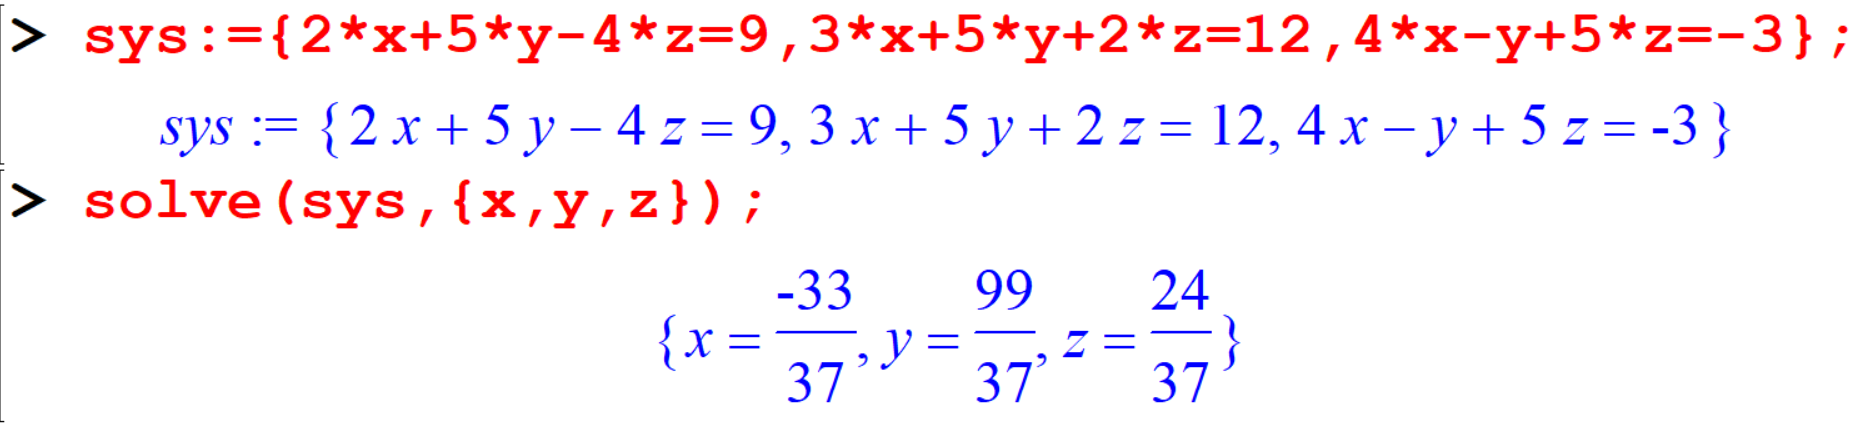
\includegraphics{figures/Lesson 5/fig4.png}

Maple will automatically use fractions, however you can force decimal answers using the \textbf{\emph{evalf}} command.

\begin{verbatim}
[> evalf(%);
\end{verbatim}

\emph{Output}:

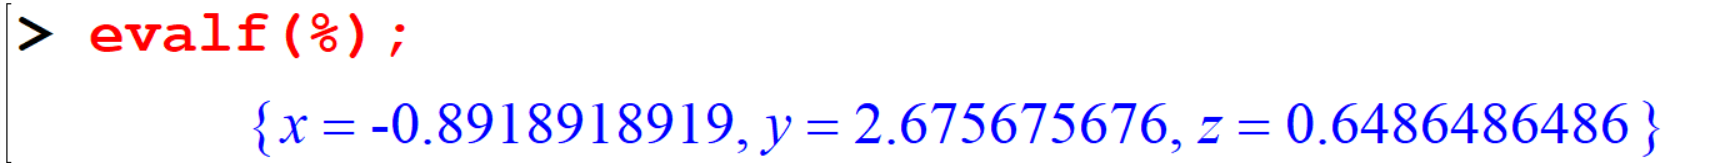
\includegraphics{figures/Lesson 5/fig5.png}

\subsection{Method II}\label{method-ii}

We can also convert the above system of equations to a matrix system.

\begin{verbatim}
[> A:=genmatrix(sys,[x,y,z],b);
[> evalm(b);
\end{verbatim}

\emph{Output}:

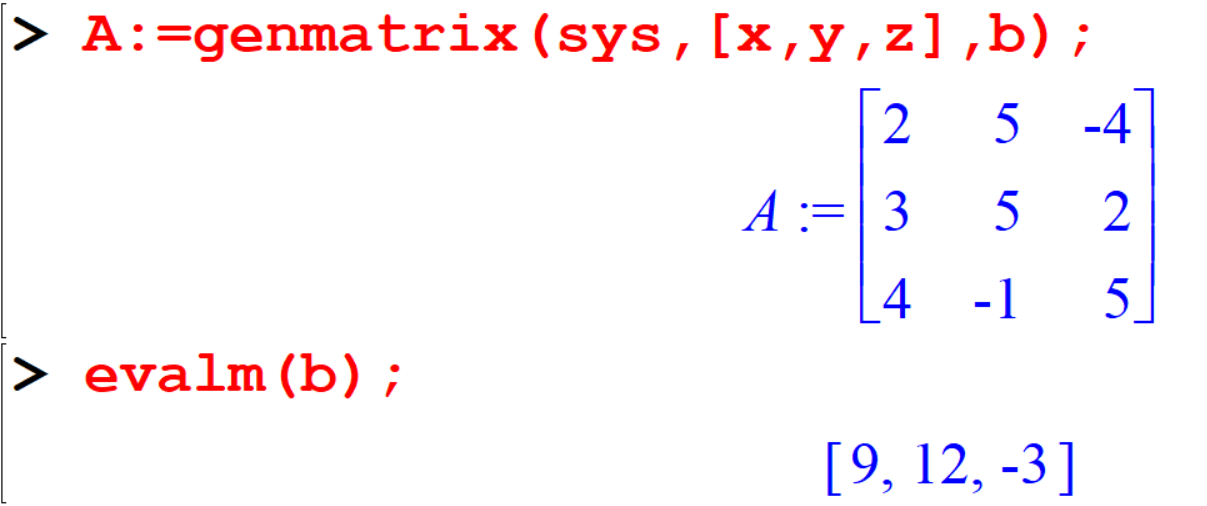
\includegraphics[width=0.7\textwidth,height=\textheight]{figures/Lesson 5/fig6.png}

In this case ,

\begin{itemize}
\tightlist
\item
  \(A\) is the coefficient matrix, and
\item
  \(b\) is vector representing the constant values.
\end{itemize}

The command \texttt{evalm(b)} evaluated \(b\) as a matrix (a vector is a \(n \times 1\) matrix).
In other words, this command simply writes out what the vector \(b\) looks like.

\begin{verbatim}
[> linsolve(A,b);
\end{verbatim}

\emph{Output}:

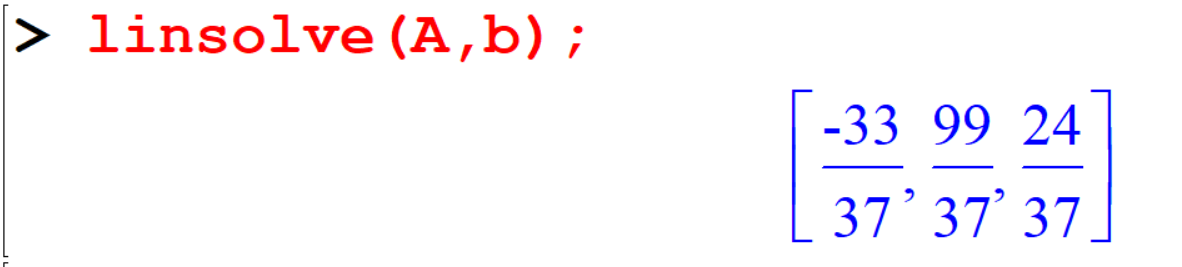
\includegraphics[width=0.7\textwidth,height=\textheight]{figures/Lesson 5/fig7.png}

\subsection{Method III}\label{method-iii}

Another way to solve a matrix equation \(Ax = b\) is to left multiply both sides by the inverse matrix \(A^{-1}\), if it exists, to get the solution \(x = A^{-1}b\).

\begin{verbatim}
[>  inverse(A);
[> evalm(inverse(A)&*b);
\end{verbatim}

\emph{Output}:

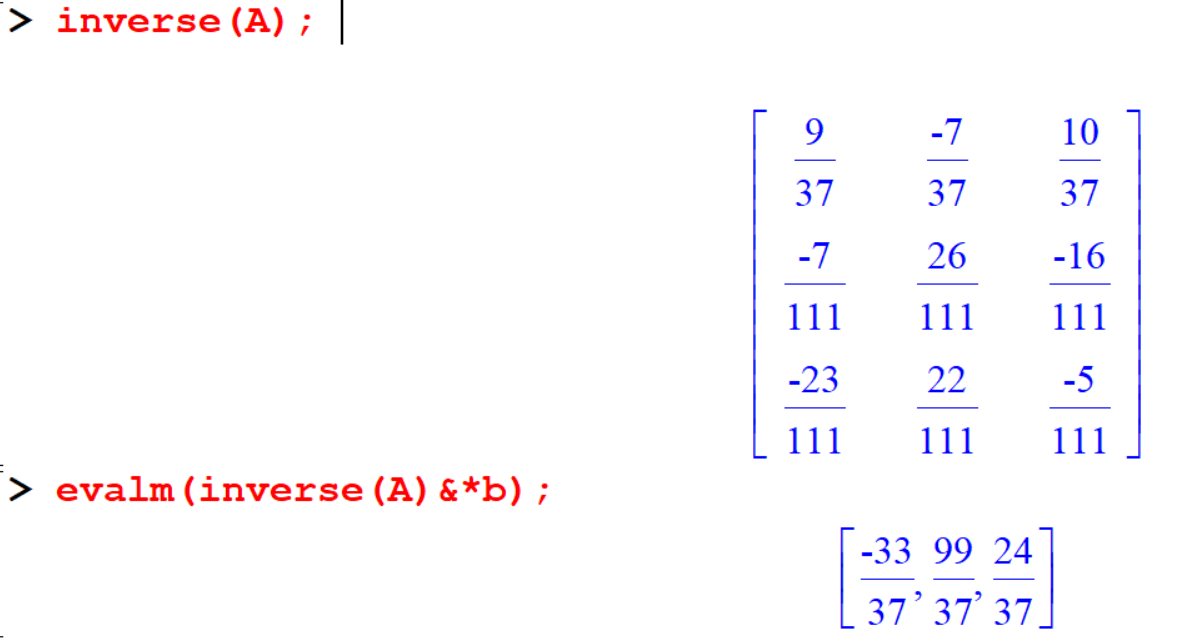
\includegraphics{figures/Lesson 5/fig8.png}

The \texttt{evalm} command forces a matrix computation and express the result.

\begin{center}\rule{0.5\linewidth}{0.5pt}\end{center}

\textbf{Dependent Systems}:

Some systems are dependent which means there are an infinite number of solutions. The form of these solutions will entail the use of parameters.
Let's look an example using two different methods; \texttt{solve} and \texttt{linsolve}.

\begin{example}
\protect\hypertarget{exm:unnamed-chunk-1}{}\label{exm:unnamed-chunk-1}\[
\begin{array}{ccccccccc}
x &-& 2y&+& z &=& &3\\
x &+& y &-& 2z&=&-&4\\
2x&-& y &-& z &=&-&1  
\end{array}
\]
\end{example}

\begin{verbatim}
[> restart;
[> with(linalg):
[> sys:={x-2*y+z=3,x+y-2*z=-4,2*x-y-z=-1};
[> solve(sys,{x,y,z});
\end{verbatim}

\emph{output}:
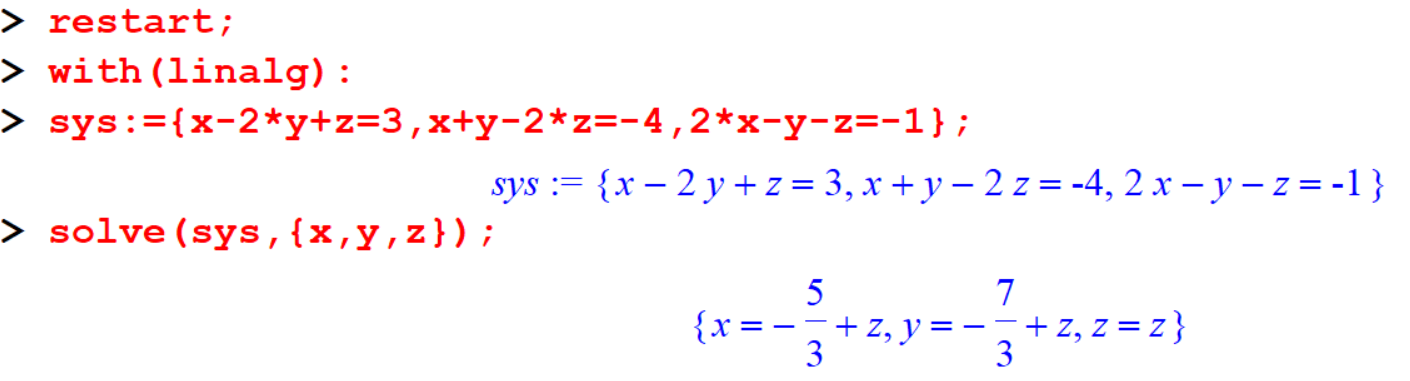
\includegraphics{figures/Lesson 5/fig9.png}

\begin{verbatim}
[> A:=genmatrix(sys,[x,y,z],b);
[> evalm(b);
[> linsolve(A,b);
\end{verbatim}

\emph{output}:

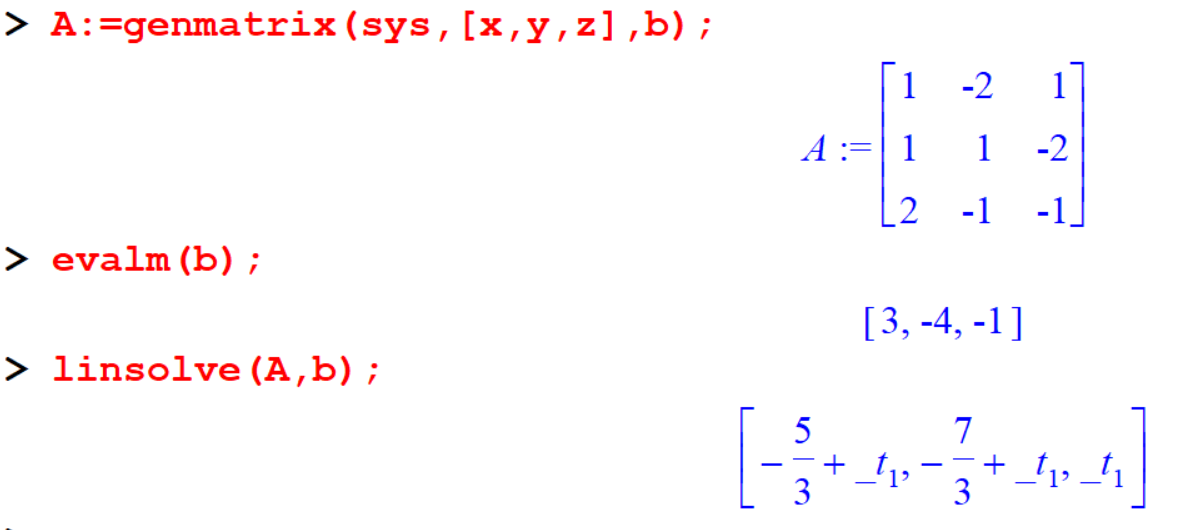
\includegraphics{figures/Lesson 5/fig10.png}

In both cases, the solution contains a parameter.
The \texttt{solve} command express it in terms actual variable used,and the \texttt{linsolve} command use the funny t character to distinguish it from a variable you might have defined yourself.

\begin{center}\rule{0.5\linewidth}{0.5pt}\end{center}

\textbf{Inconsistent System}

An Inconsistent system has no solution. Maple generally, refers to answer questions which have no answer.

\begin{example}
\protect\hypertarget{exm:unnamed-chunk-2}{}\label{exm:unnamed-chunk-2}\[
\begin{array}{ccccccccc}
x &+& y &-& 3z &= 10\\
x &+& y &-&  z &= 1\\
x &+& y &+&  z &= 8  
\end{array}
\]
\end{example}

Let's try to solve this system.

\begin{verbatim}
[> restart;
[> with(linalg):
[> sys:={x+y-3*z=10,x+y-z=1,x+y+z=8};
[> solve(sys,{x,y,z});
\end{verbatim}

\emph{Output}:

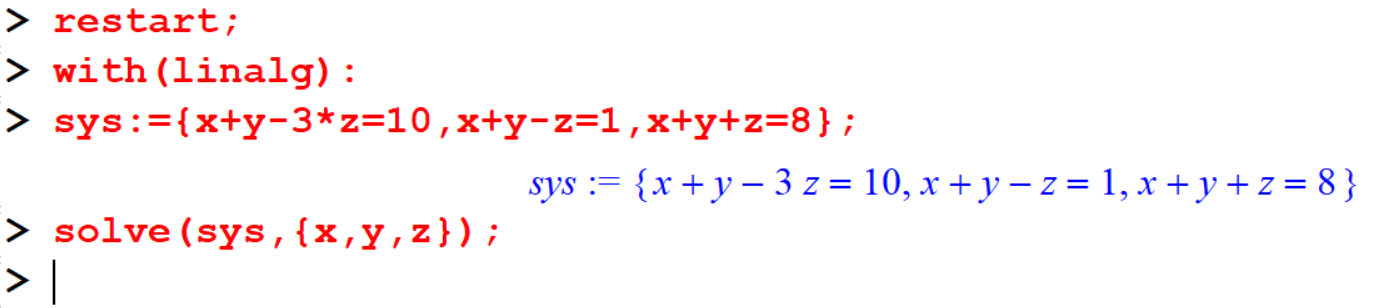
\includegraphics{figures/Lesson 5/fig11.png}

This method does not work. It does not return anything.

Let's try \texttt{linsolve} method.

\begin{verbatim}
[> A:=genmatrix(sys,[x,y,z],b);
[> linsolve(A,b);
\end{verbatim}

\emph{Output}:

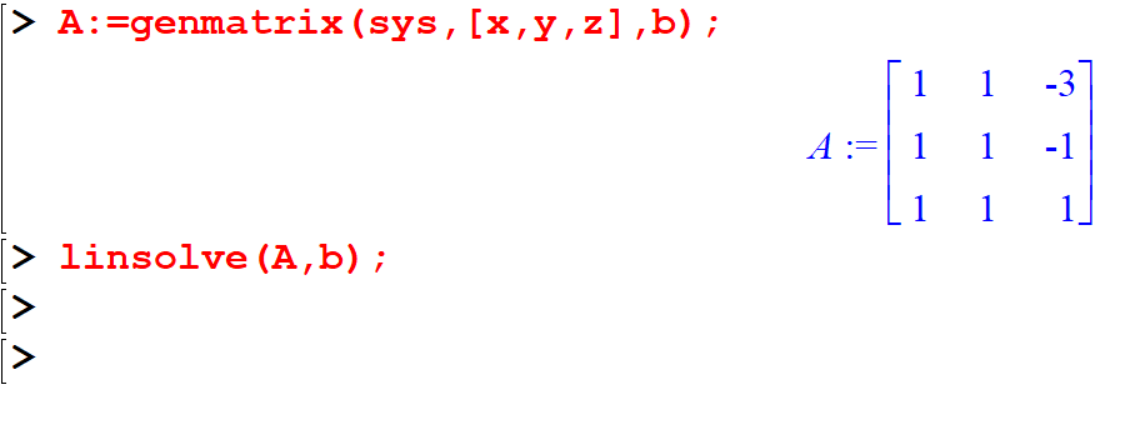
\includegraphics{figures/Lesson 5/fig12.png}

This method also does not works.

\begin{verbatim}
[> evalm(inverse(A)&*b);
\end{verbatim}

\emph{Output}:

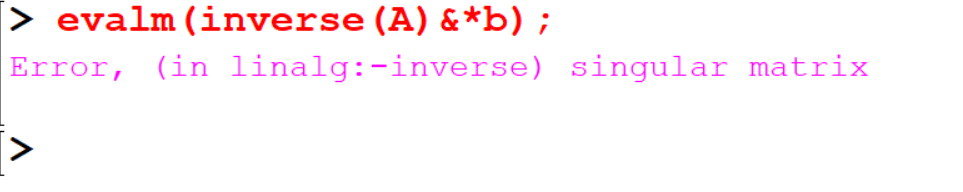
\includegraphics{figures/Lesson 5/fig13.png}

\subsubsection{Automatic Reduction}\label{automatic-reduction}

\begin{verbatim}
[> sys:={3*x+5*y+2*z=12,2*x+5*y-4*z=9,4*x-y+5*z=-3};
[> evalm(b);
[> C:=augment(A,b);
\end{verbatim}

\emph{Output}:

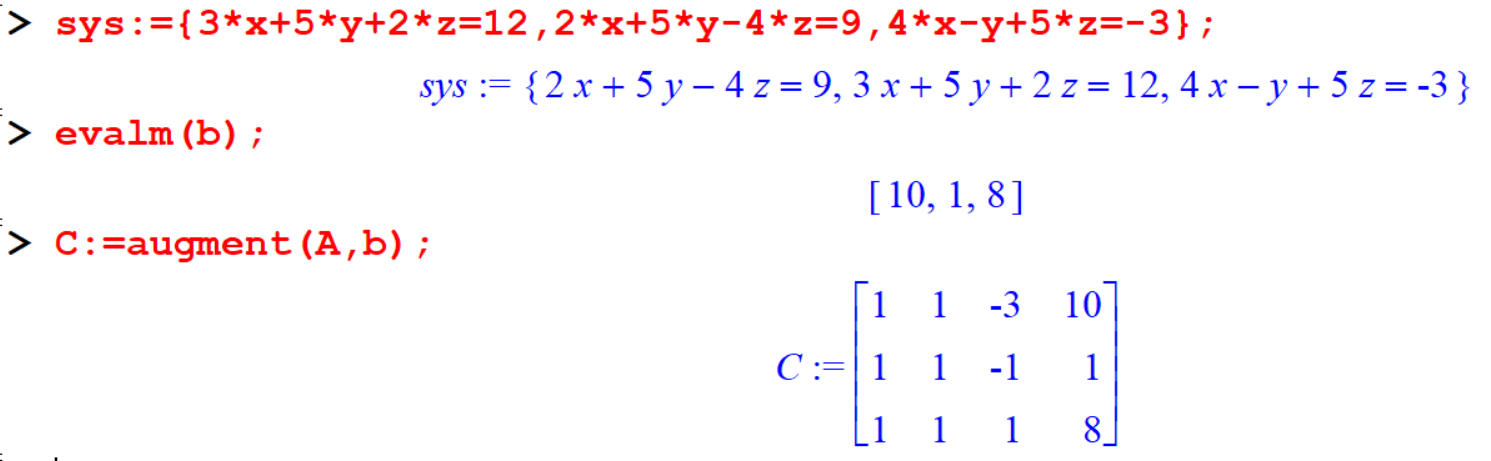
\includegraphics{figures/Lesson 5/fig14.png}

\subsection{Method IV}\label{method-iv}

An even faster method is simplifying let maple to do all the work for us. The \texttt{gausselim} command will perform all of the steps of Gaussian eliminations and reduce an augmented matrix to \textbf{row echelon form}.

\begin{verbatim}
[> sys:={3*x+5*y-2*z=12,2*x+5*y-4*z=9,4*x-y+5*z=-3};
[> A:=genmatrix(sys,[x,y,z],b);
[> evalm(b);
[> C:=augment(A,b);
[> gausselim(C);
\end{verbatim}

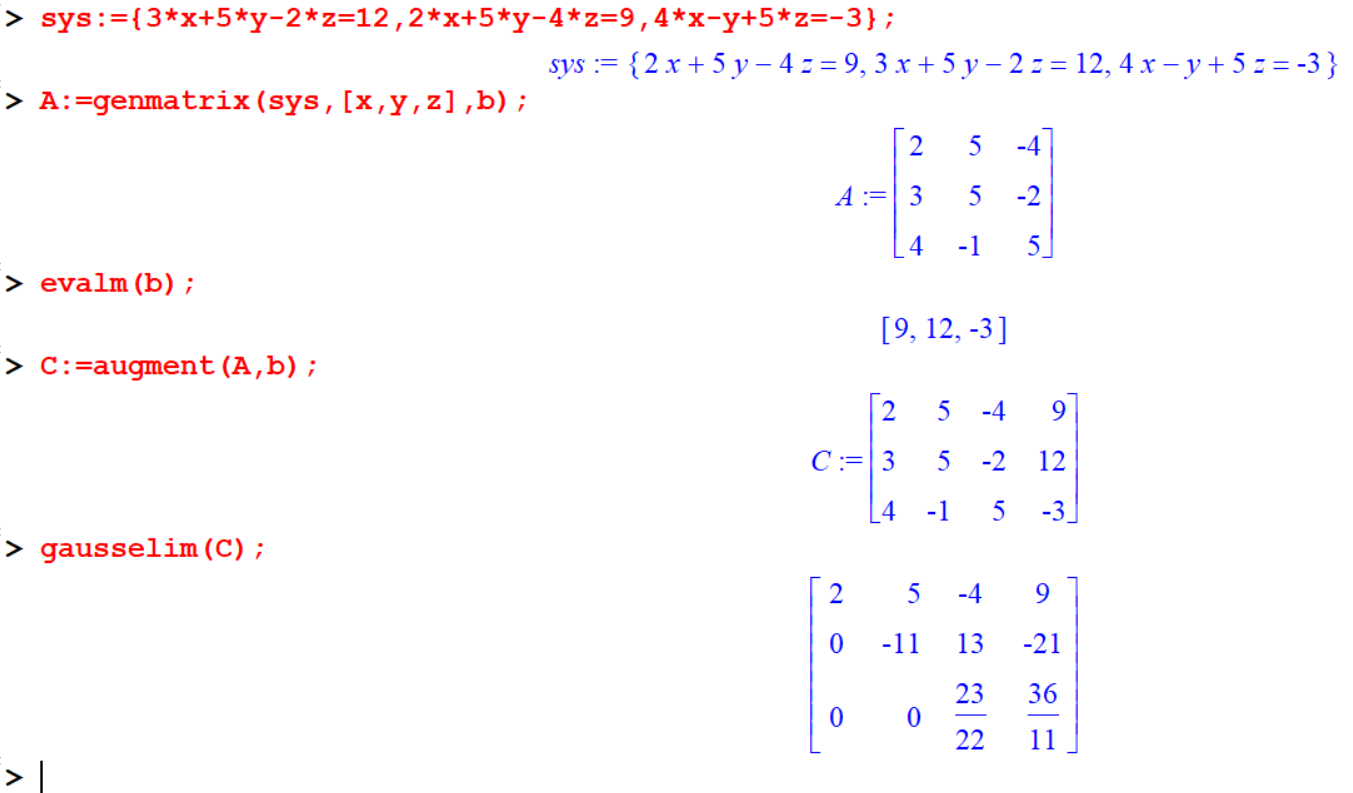
\includegraphics{figures/Lesson 5/fig15.png}

\subsection{Method V}\label{method-v}

The command \texttt{gaussjord} does the same thing.
It performs all the steps of Gauss Jordan elimination and reduces and reduces an augmented matrix into reduced row echelon form.

\begin{verbatim}
[> gaussjord(C);
\end{verbatim}

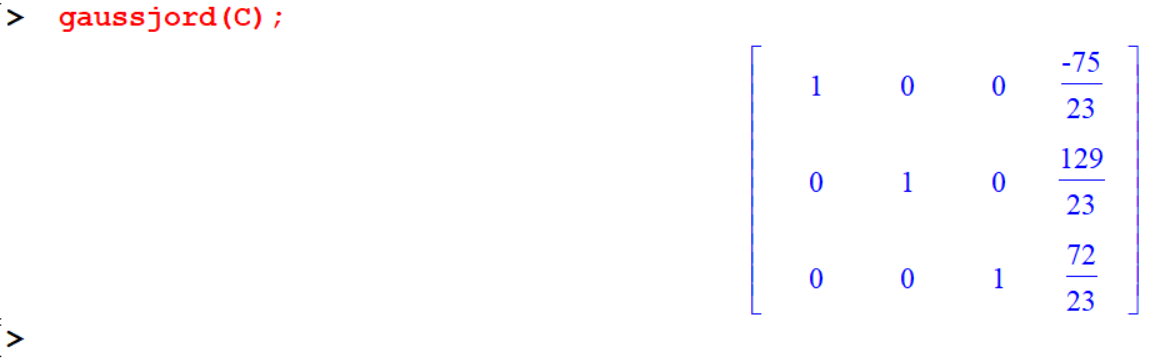
\includegraphics{figures/Lesson 5/fig16.png}

\begin{center}\rule{0.5\linewidth}{0.5pt}\end{center}

\section{Exercise}\label{exercise-5}

\begin{exercise}
\protect\hypertarget{exr:unnamed-chunk-3}{}\label{exr:unnamed-chunk-3}Solve the following system of equations.
\[
\begin{array}{ccccccc}
x_1  &+& 2x_2 &+& 3x_3 &= 9 \\
2x_1 &-& x_2  &+& x_3  &= 8 \\
3x_1 & &      &-& x_3&= 3
\end{array}
\]
\end{exercise}

\begin{exercise}
\protect\hypertarget{exr:unnamed-chunk-4}{}\label{exr:unnamed-chunk-4}

A small manufacturing plant makes three types of inflatable boats: one-person, two-person, and four-person models.
Each boat requires the services of three departments, as listed in the table.
The cutting, assembly, and packaging departments have available a maximum of 380, 330, and 120 labor hours per week, respectively.

\begin{longtable}[]{@{}
  >{\centering\arraybackslash}p{(\columnwidth - 6\tabcolsep) * \real{0.2464}}
  >{\centering\arraybackslash}p{(\columnwidth - 6\tabcolsep) * \real{0.2464}}
  >{\centering\arraybackslash}p{(\columnwidth - 6\tabcolsep) * \real{0.2464}}
  >{\centering\arraybackslash}p{(\columnwidth - 6\tabcolsep) * \real{0.2609}}@{}}
\toprule\noalign{}
\begin{minipage}[b]{\linewidth}\centering
Department
\end{minipage} & \begin{minipage}[b]{\linewidth}\centering
One Person Boat
\end{minipage} & \begin{minipage}[b]{\linewidth}\centering
Two-Person Boat
\end{minipage} & \begin{minipage}[b]{\linewidth}\centering
Four-Person Boat
\end{minipage} \\
\midrule\noalign{}
\endhead
\bottomrule\noalign{}
\endlastfoot
Cutting & 0.5 hr & 1.0 hr & 1.5 hr \\
Assembling & 0.6 hr & 0.9 hr & 1.2 hr \\
Packaging & 0.2 hr & 0.3 hr & 0.5 hr \\
\end{longtable}

\begin{enumerate}
\def\labelenumi{(\Alph{enumi})}
\tightlist
\item
  How many boats of each type must be produced each week for the plant to operate at full capacity?
\item
  How is the production schedule in part A affected if the packaging department is no longer used?
\item
  How is the production schedule in part A affected if the four-person boat is no longer produced?
\end{enumerate}

\end{exercise}

\chapter{Intergration}\label{intergration}

Placeholder

\section{Indefinite Integration}\label{indefinite-integration}

\section{Definite Integration}\label{definite-integration}

\section{Integration by Parts}\label{integration-by-parts}

\section{Substitutions}\label{substitutions}

\section{Multiple Integration}\label{multiple-integration}

\subsection{Double integration (Area calculation)}\label{double-integration-area-calculation}

\subsection{Triple integration (Volume Calculation)}\label{triple-integration-volume-calculation}

\section{Exercise}\label{exercise-6}

\section{Computing the area from the integral}\label{computing-the-area-from-the-integral}

\section{Exercise}\label{exercise-7}

\chapter{Differential Equations}\label{differential-equations}

Placeholder

\section{Introduction to differential equations}\label{introduction-to-differential-equations}

\subsection{Exercise}\label{exercise-8}

\section{Higher derivatives}\label{higher-derivatives}

\subsection{Method 1}\label{method-1}

\subsection{Method 2}\label{method-2}

\subsection{Exercise}\label{exercise-9}

\section{Homogenous Equations}\label{homogenous-equations}

\section{Solving Differential Equations}\label{solving-differential-equations}

\section{Direction Fields}\label{direction-fields}

\subsection{Exercise}\label{exercise-10}

\chapter{Equations and Functions}\label{equations-and-functions}

Placeholder

\section{Solving Equations}\label{solving-equations}

\section{Equations with multiple unknowns}\label{equations-with-multiple-unknowns}

\section{Functions}\label{functions}

\subsection{Defining functions}\label{defining-functions}

\subsection{Function Operations and Compositions}\label{function-operations-and-compositions}

\subsection{Composition of functions}\label{composition-of-functions}

\section{Trigonometry with Maple}\label{trigonometry-with-maple}

\section{Inverse trigonometric functions}\label{inverse-trigonometric-functions}

\section{Exercise}\label{exercise-11}

\chapter{Plots}\label{plots}

\textbf{Maple Packages}

In Maple we can use various packages for special applications. In order to use a package, you have to load the package first using the \texttt{with} command.

\textbf{Example}\\
\texttt{\textgreater{}\ with(student):}\strut \\
\texttt{\textgreater{}\ with(linalg):}

So, when you are dealing with plots, you have to load the package \texttt{plot}.

\begin{verbatim}
 > with(plots):
\end{verbatim}

\section{Basic Graphs}\label{basic-graphs}

Using the plot command you can graph a function. You have to give the range of values for \(x\) otherwise Maple will use the default range.

\section{Multiple Graphs}\label{multiple-graphs}

If you want to compare plots, you can have two or more plot windows open at the same time or you can plot more than one curve on the same set of axes. The plot command offers options which control the number of points at which the function is plotted, the number of
tick marks on the axes and the placing of titles on the graph. Read the help page on plot to find out about these options.

\chapter{Introduction to Maple}\label{introduction-to-maple-1}

Placeholder

\section{What is Maple?}\label{what-is-maple-1}

\section{Using a Maple Worksheet}\label{using-a-maple-worksheet-1}

\section{Entering Maple Commands}\label{entering-maple-commands-1}

\section{Arithmetic operations}\label{arithmetic-operations-1}

\section{Operations}\label{operations-1}

\subsection{Exercises}\label{exercises-2}

\section{Shortcut to retyping}\label{shortcut-to-retyping-1}

\section{Fractions and Decimals}\label{fractions-and-decimals-1}

\section{Roots}\label{roots-1}

\subsection{Exercise}\label{exercise-12}

\section{Pi Vs pi}\label{pi-vs-pi-1}

\section{Rational Numbers}\label{rational-numbers-1}

\subsection{Exercises}\label{exercises-3}

\section{Complex Numbers}\label{complex-numbers-1}

\subsection{Exercise}\label{exercise-13}

\section{MAPLE Help}\label{maple-help-1}

  \bibliography{book.bib,packages.bib}

\end{document}
